\documentclass[a4paper,12pt]{article}
\usepackage{a4wide}
\usepackage[T1]{fontenc}
\usepackage{lmodern}
\usepackage{textcomp} 
\usepackage[utf8]{inputenc}
\usepackage{xcolor}
\usepackage[czech,english]{babel}
\usepackage[pdftex, final]{graphicx}
% \usepackage[pdftex, final, colorlinks=true]{hyperref}
\usepackage{verbatim}
\usepackage{alltt}
\usepackage{paralist}
\usepackage{mdwlist}
\usepackage{subfig}
\usepackage[final]{pdfpages}
%\usepackage[hyphens]{url}
%\PassOptionsToPackage{hyphens}{url}

\usepackage[final,pdftex,colorlinks=false,breaklinks=true]{hyperref}
\usepackage[hyphenbreaks]{breakurl}

%%%%%%%%%%%%%%%%%%%%%%%%%
% pro podmineny preklad
% false je defaultně


% \newif\ifbc % Pouze do bakalářské práce
%  \bctrue

%%%%%%%%%% fancy %%%%%%%%%%%
\usepackage{fancyhdr}

\fancyhead[L]{ČVUT v Praze}

\setlength{\headheight}{16pt}

% \usepackage{stdpage}


%%%%%%%%%%%% rozmery %%%%%%%%%%%%%%%%%%
\usepackage[%
%top=40mm,
%bottom=35mm,
%left=40mm,
%right=30mm
top=40mm,
bottom=35mm,
left=35mm,
right=25mm
]{geometry}


\renewcommand\baselinestretch{1.3}
\parskip=0.8ex plus 0.4ex minus 0.1 ex

\newcommand{\klicslova}[2]{\noindent\textbf{#1: }#2}
\newcommand{\modul}[1]{\emph{#1}}
\author{Štěpán Turek}
% \pagecolor{darkGrey}
\newcommand{\necislovana}[1]{%
\phantomsection
\addcontentsline{toc}{section}{#1}
\section*{#1}
\markboth{\uppercase{#1}}{}
}

%%%%%%%%%%%%%%%%%%%%%%%%%%%%%%
\begin{document}
\pagestyle{empty}

\begin{center}
%napisy
\newcommand{\napisCVUT}{České vysoké učení technické v Praze}
\newcommand{\napisFS}{Fakulta stavební}
\newcommand{\napisObor}{Obor geoinformatika}
\newcommand{\napisKatedra}{Katedra mapování a kartografie}
\newcommand{\napisVedouci}{Ing. Martin Landa}
\newcommand{\napisAutor}{Štěpán Turek}
\newcommand{\napisDatum}{Praha 2012}
\newcommand{\napisNazevI}{Implementace podpory WMS }
\newcommand{\napisNazevII}{do programů GRASS GIS a SAGA GIS}
\newcommand{\napisNazevAjI}{Implementation of WMS support}
\newcommand{\napisNazevAjII}{in GRASS GIS and SAGA GIS}
\newcommand{\napisBakalarka}{Bakalářská práce}
\newcommand{\napisPraha}{Praha 2012}
%
% prikazy
%\newcommand{\velka}[1]{\uppercase{#1}}
\newcommand{\velka}[1]{\textsc{#1}}
%
% 
\newif\ifpatitul
\patitultrue

\ifpatitul
{\Large\velka{\napisCVUT}}\\
\velka{\Large\napisFS}\\
\vfill
{\LARGE\velka{\napisBakalarka}}
\vfill
{\large\napisPraha\hfill\napisAutor}
\newpage
\fi%patitul


{\Large\velka{\napisCVUT}}\\
{\Large\velka{\napisFS}}\\
{\Large\velka{\napisObor}}
\vfill

\includegraphics[width=3cm]{logo_cvut_cb} %~
\vfill
{\Large\velka{\napisBakalarka}}\\
{\Large\velka{\napisNazevI\\
\napisNazevII}}\\
{\large\velka{\napisNazevAjI\\
\napisNazevAjII}}
\vfill
{\large%
Vedoucí práce: \napisVedouci\\
\napisKatedra\\
\bigskip
\napisDatum\hfill\napisAutor}
\end{center}

\newpage
\definecolor{navodotisk}{RGB}{10,10,10}
\newcommand{\vlozZadani}{%
\Huge\textcolor{navodotisk}{\textsf{\textbf{ZDE VLOŽIT ORIGINÁLNÍ ZADÁNÍ}}}%
}
%%%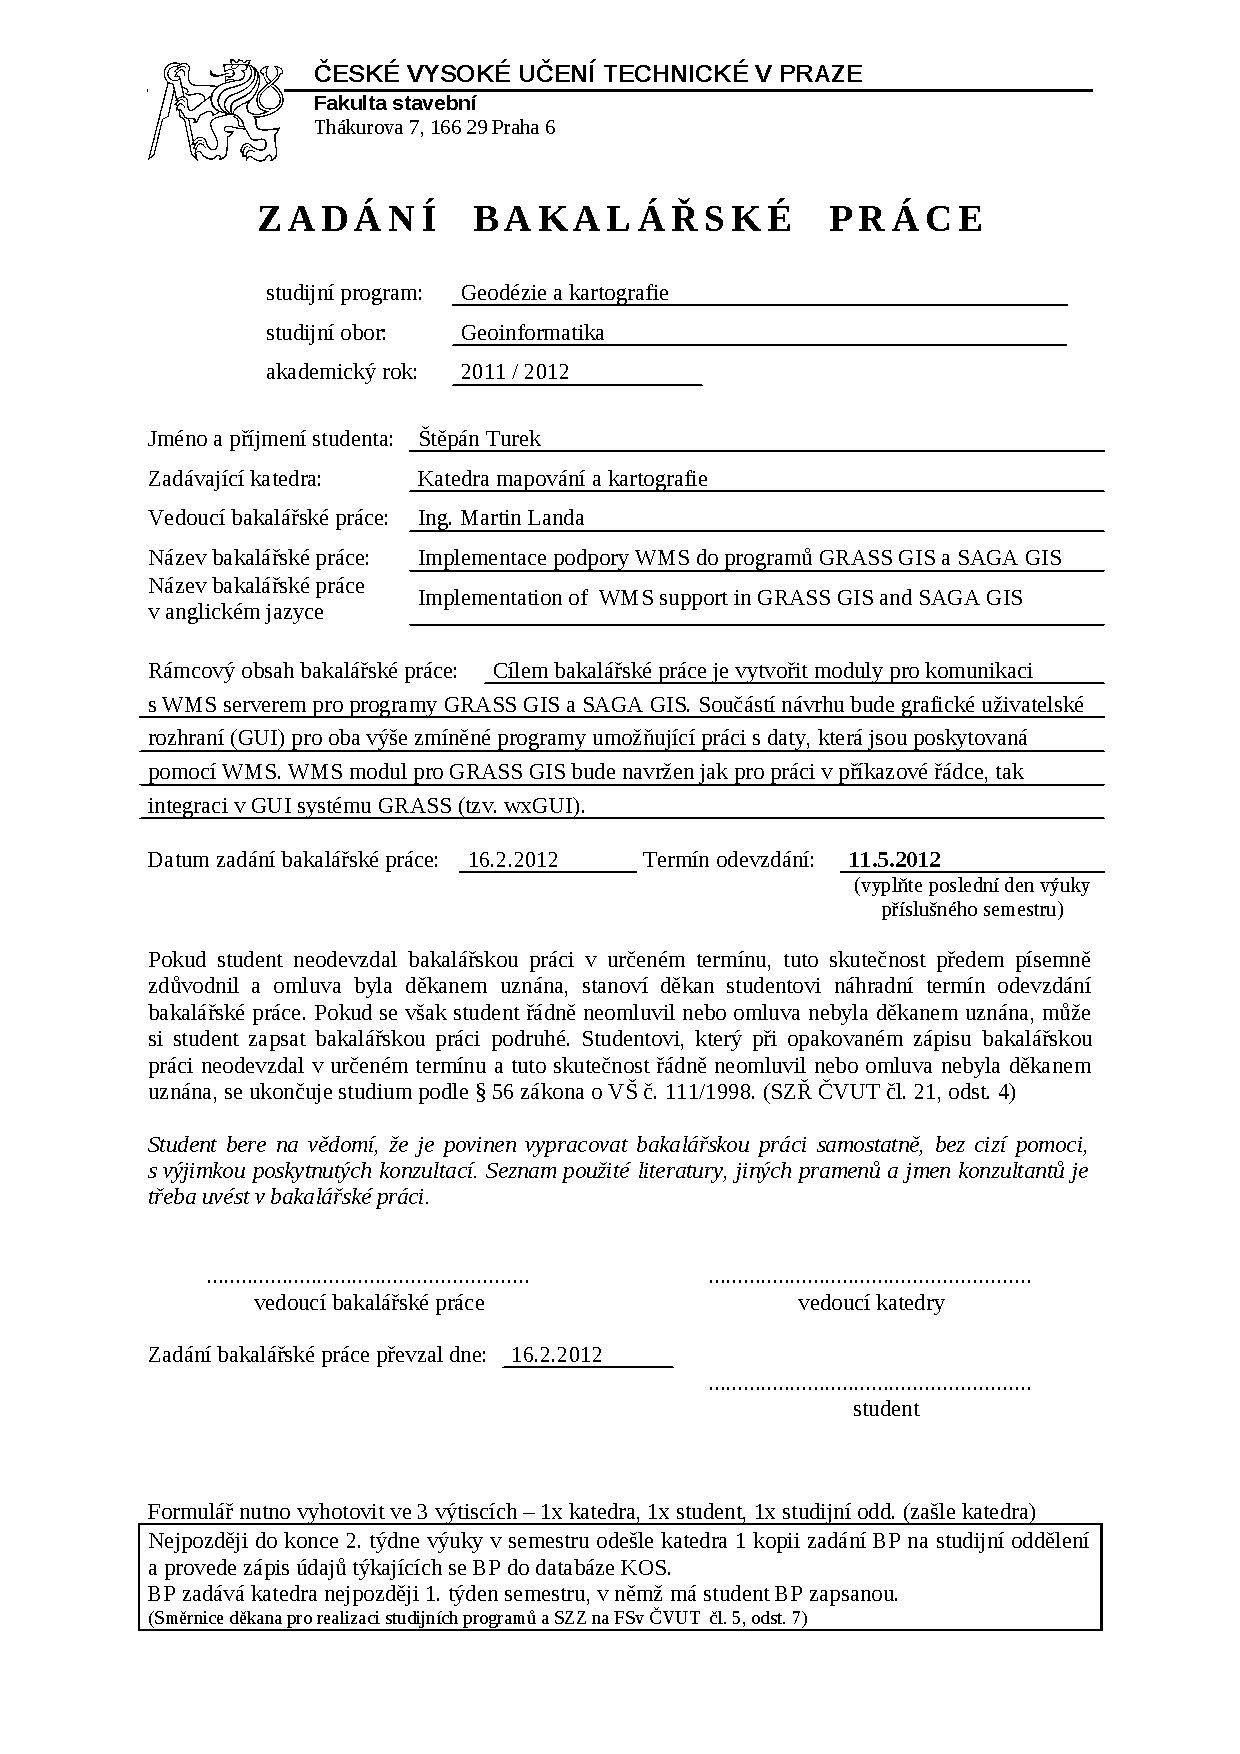
\includepdf[picturecommand={\put(100,200){\vlozZadani}}]{zadani}
 % resi si zalomeni sam





\begin{abstract}

\bigskip

\klicslova{Klíčová slova}{GIS, GRASS, SAGA}

\end{abstract}

\selectlanguage{english}
\begin{abstract}

\bigskip

\klicslova{Keywords}{GIS, GRASS, SAGA}

\end{abstract}
\selectlanguage{czech}


\newpage
\newcommand{\odsaditodzhora}{\hskip1pt\vfill}

\odsaditodzhora
\noindent Prohlášení



\begin{flushleft}
\begin{tabular}{cp{0.3\textwidth}c}
V Praze dne .................
& 
&
..................................
\\
&&
(podpis autora)
\end{tabular}

\end{flushleft}
\newpage

\odsaditodzhora
\noindent Poděkování


\newpage

\newpage
\tableofcontents


\newpage
\pagestyle{fancy}

\necislovana{Úvod}



GRASS GIS (\url{http://grass.osgeo.org}) je geografický informační systém, šířený  pod svobodnou licencí GNU GPL.  
Historie GRASS GIS sahá do roku 1982. V tomto roce americká armáda začala vyvíjet software, který by ji pomohl se správou rozsáhlých oblastí z hlediska ochrany 
životního prostředí. Příčinou byla nová, přísnější legislativa ve vztahu k tomuto odvětví, která kladla na majitelé pozemků větší požadavky a americká armáda patří mezi jedny z největších vlastníku půdy v USA.
 
Významným milníkem pro GRASS byl rok 1995, kdy se americká armáda z toho projektu stáhla a kolem GRASS se začala rodit komunita dobrovolníků. 
Dnes je komunita vývojářů rozprostřena po celém světě, z nichž se většina rekrutuje z univerzit a výzkumných ústavů. 

GRASS je jeden z nejrobustnějších svobodných GIS software. Umožňuje pracovat s vektorovými a rastrovými daty.
Jelikož se GRASS vyvíjí již 25 let, jedním z dědictví takto dlouhého vývoje je, že jeho jádro je napsáno procedurálně v jazyce C. 
V poslední době je snaha vývojářů učinit GRASS použitelnější pro méně pokročilé uživatele. Z tohoto důvodu bylo vyvinuto nové GUI, které se intenzivně rozvijí. 
Funkcionality GRASS GIS jsou do programu implementovány v podobě modulů. Moduly jsou do programu integrovány pomocí API, které existuje v C a Python verzi.

SAGA GIS (\url{http://www.saga-gis.org/}) je menší open source projekt, jehož vývoj začal na
 univerzitě v Goettingenu kolem roku 2004. Nyní je tento program šířen pod  licencí GNU GPL. Vývojářská 
komunita je mezinárodní s těžištěm na domovské universitě. Hlavní síla SAGA GIS spočívá v práci s rastrovými daty. Program je schopen pracovat i s daty vektorovými. 
SAGA GIS je napsán v jazyce  C++ a je rovněž koncipován modulárně. Moduly jsou do jádra integrovány pomocí API v jazyce C++.

Web Map Service (WMS) je standard\footnote{\url{http://www.opengeospatial.org/standards/wms}}, který definuje rozhraní mezi klientem 
a serverem pro získávání georeferencovaných dat v rastrových formátech \footnote{ Vektorová data ve formátu SVG nebo CGM.} (např. JPEG, TIFF, PNG...). 
Jde o otevřený standard vyvíjený organizací OGC.\footnote{\url{http://www.opengeospatial.org/}}.  


\newpage
\section{Stručný úvod do WMS}

Komunikace mezi klientem a serverem probíhá pomocí protokolu HTTP, kdy klient zašle serveru požadavek, 
server požadavek zpracuje a  zašle klientu soubor s odpovědí, což může být rastr ve formátu definovaném klientem, nebo soubor s metadaty.

WMS standard je definován v několika verzích:

\begin{table}[h]
\centering
\begin{tabular}{|c|c|c|c|}      \hline
  Číslo verze  & Rok vydání  \\ \hline
  1.0.0        &  2000       \\ \hline
  1.1.0        &  2001       \\ \hline
  1.1.1        &  2002       \\ \hline
  1.3.0        &  2004       \\ \hline
\end{tabular}
\caption{Verze WMS}
\label{tab:verze}
\end{table}

V dnešní době téměř všechny servery podporují verze 1.3.0 a 1.1.1. Protože
změny ve verzi 1.3.0 nejsou uvedeny ve standardu a na internetu jsou těžko dohledatelné, jsou popsány v příloze této práce [TODO odkaz].


\subsection{Komunikace klient-server}


Požadavek klienta na WMS server může být zaslán pomocí dotazovacích metod GET a POST protokolu HTTP. Pomocí těchto metod je klient schopen
serveru předat parametry, na základě kterých server vytvoří odpověď. WMS standard vyžaduje podporu metody GET, zatímco podpora metody POST je volitelná. 

\subsubsection{HTTP GET}

Metoda GET předává parametry jako součást URL. URL adresa je řetězec znaků reprezentující adresu zdroje informací. Tento řetězec má pevně danou strukturu:
	
\begin{alltt}\footnotesize
	protokol://SERVER: port / cesta k dokumentu ? parametry
\end{alltt}
	
Tomuto odpovídá tento příklad WMS dotazu metodou GET:

\begin{alltt}\footnotesize
\url{http://wms.cuzk.cz:80/wms.asp?REQUEST=GetCapabilities&VERSION=1.1.1}
\end{alltt}

\newpage

Protože port číslo 80 pro protokol HTTP je implicitní, není třeba jej zadávat.   
Aby server byl schopen rozpoznat jednotlivé části URL adresy, jsou určeny znaky (viz. tab \ref{tab:myfirsttable}) se speciálními funkcemi.

\begin{table}[h]
\centering
\begin{tabular}{|c|l|}      \hline
  Znak      &    Funkce				\\ \hline
   ?        &  Začátek řetězce parametrů.      	\\ \hline
   \&       &  Oddělovač parametrů.   		\\ \hline
   =        &  Oddělovač názvu parametru a jeho hodnoty.    \\ \hline
   ,        &  Oddělovač jednotlivých položek, pokud parametr obsahuje více hodnot\\ \hline
   +        &  Reprezentuje mezeru. 	\\ \hline
\end{tabular}
\caption{Znaky v URL se speciální funkcí}
\label{tab:myfirsttable}
\end{table}

Pokud je potřeba v URL uvést tyto vyhrazené znaky, lze použít URL kódování\footnote{\url{hhttp://www.w3schools.com/tags/ref_urlencode.asp}}.

\subsubsection{HTTP POST}

Metoda POST neposílá parametry v URL adrese, ale přenáší je v těle POST zprávy.


\subsection{Komunikace server-klient}

Odpovědí serveru na WMS dotaz je soubor, který se odesílá protokolem Multipurpose Internet Mail Extensions\footnote{\url{http://mgrand.home.mindspring.com/mime.html}}. Tento protokol umožňuje zasílat soubory pomocí protokolu HTTP.


\subsection{Fungování WMS v praxi}

 
Nejčastěji uživatel získává data z WMS serveru pomocí klienta, který je součástí GIS nebo jiného programu. Každý klient na pozadí vytváří WMS dotazy a jejich 
tvorba je v této kapitole popsána na reálných příkladech. 


\newpage
Jediné, co je potřeba znát pro zahájení komunikace s WMS serverem, je jeho URL. V tomto případě:
\begin{alltt}\footnotesize
\url{http://geoportal.cuzk.cz/WMS_ZABAGED_PUB/WMService.aspx}
\end{alltt}

Nyní musí klient vytvořit dotaz typu GetCapabilities, aby zjistil informace o datech, která server poskytuje a o parametrech pro ostatní WMS dotazy (GetMap a GetFeatureInfo).
Toto učiní přidáním parametrů k URL adrese WMS serveru:

\newcommand{\CUZKgetCap}{http://geoportal.cuzk.cz/WMS_ZABAGED_PUB/WMService.aspx?SERVICE=WMS&REQUEST=GetCapabilities&VERSION=1.3.0}
\begin{alltt}\footnotesize
\href{\CUZKgetCap}{http://geoportal.cuzk.cz/WMS_ZABAGED_PUB/WMService.aspx?}
\href{\CUZKgetCap}{SERVICE=WMS&REQUEST=GetCapabilities&VERSION=1.3.0}
\end{alltt}

 Dotaz typu GetCapabilities obsahuje parametry, které jsou společné všem typům WMS dotazů, protože definují způsob komunikace.
\begin{itemize}
  \item Parametr SERVICE sděluje serveru, že se jedná o WMS dotaz. 
  \item Parametr REQUEST charakterizuje typ dotazu. 
  \item Parametr VERSION popisuje v jaké verzi WMS standardu je dotaz sestaven.
\end{itemize}

Aby byl server schopen správně zpracovat WMS dotazy, musí se s klientem dohodnout na verzi WMS, ve které bude probíhat následná komunikace.
Toto je součástí dotazu typu GetCapabilities. Pokud není v dotazu GetCapabilities uveden parametr VERSION, server odpoví ve formátu nejvyšší podporované verze. 
Pokud klient explicitně požaduje určitou verzi, server odpoví v dané verzi, pokud ji podporuje. Jak bylo výše zmíněno, dnes naprostá většina serverů podporuje 
verze WMS standardu 1.1.1 a 1.3.0. Pokud klient podporuje tyto dvě verze, problém s nekompatibilitou v podstatě odpadá. Parametr VERSION může být vynechán pouze u GetCapabilities dotazu u ostatních typů dotazů musí být vždy specifikován.

Na tento dotaz server vrátí soubor ve formátu XML. 

Informace o verzi je uvedena jako atribut úvodního kořenového elementu:
\begin{alltt}\footnotesize
<WMS_Capabilities...    ...version="1.3.0">
\end{alltt}

Přímými potomky kořenového elementu jsou elementy <Service> a <Capability>.

Element  <Service> obsahuje informace o WMS Serveru a poskytovateli dat.
Druhý element <Capability> je mnohem důležitější, protože poskytuje všechny informace, které jsou potřeba pro další komunikaci s WMS serverem.

\begin{alltt}\footnotesize
<Capability>
    <Request>
          ...
       <GetMap>
            <Format>image/png</Format>
            <Format>image/jpeg</Format>
          ...
       </GetMap>	
       <GetFeatureInfo>
            <Format>text/html</Format>
            <Format>text/xml</Format>
              ...
       </GetFeatureInfo>
           ....
\end{alltt}
V této částí jsou uvedeny formáty odpovědí ve tvaru protokolu MIME pro dotaz typu GetMap a GetFeatureInfo. V tomto případě WMS server poskytuje  mapy jako rastry ve formátu PNG, JPEG a na 
dotaz typu GetFeatureInfo může vrátit odpověď ve formátu HTML nebo XML.  

Velmi důležitý je element <Layer>, který obsahuje informace o mapové vrstvě. Všechny vrstvy jsou uspořádány do stromové struktury s jedním kořenovým elementem.

\begin{alltt}\footnotesize
<Capability>
    ...
  <Layer>
   <Title>ZABAGED</Title>
     <CRS>EPSG:3035</CRS>
     <CRS>EPSG:3034</CRS>
     <CRS>EPSG:4326</CRS>
      ...
     <BoundingBox CRS="EPSG:3035" minx="4434628.0972282" miny="2778319.58676976"
                                  maxx="4987359.29769667" maxy="3190250.19895492"/>
     <BoundingBox CRS="EPSG:3034" minx="4109720.95957183" miny="2382975.60863023"
                                  maxx="4643932.77142764" maxy="2780500.92255097"/>
      ...
\end{alltt}

Zde je uveden název kořenové vrstvy <Title> a projekce <CRS> v nichž je dostupná. Název vrstvy se uvádí pomocí elementů <Title> a <Name>. Element
<Title> je název vrstvy ve formátu pro člověka pochopitelném a má pouze informativní charakter, zatímco element <Name> slouží jako unikátní klíč, 
pod kterým je možné danou vrstvu jednoznačně identifikovat v rámci WMS serveru. Jelikož kořenová vrstva nemá element <Name>, není možné poslat požadavek na data této vrstvy. Vrstvy, které neposkytují 
žádná data, se uvádí z důvodu dědičnosti. 

Jelikož projekce je atribut, který je v rámci stromu vrstev děděn a v příkladu jsou uvedeny atributy kořenového elementu <Layer>, jsou všechny vrstvy tohoto serveru dostupné v těchto projekcích.
Jakákoliv vrstva v tomto stromu může mít definovány další projekce, které budou děděny všemi jejími následovníky ve stromu. 

Element <BoundingBox> reprezentuje obdélník definovaný minimálními a maximálními souřadnicemi v systému projekce uvedené v atributu CRS, který vymezuje rozsah poskytovaných dat. 
Tento element se také ve stromu dědí, pokud je však v potomcích vrstvy nově defininován pro stejnou projekci, nahrazuje děděný element.

 Právě dědičnost je důvodem, proč jsou vrstvy uspořádány do stromové struktury. Díky této struktuře není potřeba v tomto případě u každé vrstvy
uvádět všech 16 souřadnicových systému a obdélníků, čímž dochází k úspoře dat, která jsou přenášena mezi serverem a klientem a také k větší přehlednosti a stručnosti XML souboru.

\newpage

\begin{alltt}\footnotesize
<Capability>
  <Layer>
    <Title>Kořenová vrstva bez dat, chybí name></Title>
    <Layer>
      <Layer>
        <Title>Vrstva č. 1</Title>
        <Name>vrstva1</Name>
      </Layer>
    <Layer>
    <Layer>
      <Layer>
        <Title>Vrstva č. 2</Title>
        <Name>vrstva2</Name>
        <Layer>
          <Title>Vrstva č. 3</Title>
          <Name>vrstva3</Name>
        </Layer>
        <Layer>
          <Title>Vrstva č. 4</Title>
          <Name>vrstva4</Name>
        </Layer>
      </Layer>
    </Layer>
</Capability>
\end{alltt}



Tato delší ukázka ilustruje uspořádání vrstev ve stromové struktuře. Kořenová vrstva se větví v první úrovní  na vrstvy vrstva1, 
vrstva2. Vrstvy vrstva1, vrstva3 a vrstva4 jsou tzv. listy stromu. Takto se nazývají elementy ve stromové struktuře, které nemají žádné potomky. 

\begin{alltt}\footnotesize
<Layer queryable="0" opaque="false" noSubsets="0">
    <Name>GR_CR4</Name>
    <Title>MČR 1 : 1 000 000</Title>
    <Style>
        <Name>Default</Name>
        <Title>Default</Title>
          ...
    </Style>
</Layer>
\end{alltt}


Každá vrstva reprezentuje určitá data, která mohou být zobrazená rozličnými způsoby. Způsob zobrazení definuje element <Style>. V tomto případě  je pro vrstvu MČR 1 : 1 000 000 
dostupný pouze jeden styl. Vztah elementů <Name> a <Title> u <Style> je stejný jako v elementu <Layer>.

Díky dotazu GetCapabilities získá klient všechny potřebné informace ke stažení dat z WMS serveru. 
Toto provede pomocí dotazu typu GetMap, v tomto tvaru:



\newcommand{\CUZKgetMap}{http://geoportal.cuzk.cz/WMS_ZABAGED_PUB/WMService.aspx?SERVICE=WMS&REQUEST=GetMap&VERSION=1.3.0&LAYERS=GR_CR4&STYLES=Default&FORMAT=image/png&CRS=EPSG:4326&BBOX=48.093144621684,11.6163532829661,51.4980192528993,19.0628256634265&WIDTH=800&HEIGHT=600}
\begin{alltt}\footnotesize
\href{\CUZKgetMap}{http://geoportal.cuzk.cz/WMS\_ZABAGED\_PUB/WMService.aspx?}
\href{\CUZKgetMap}{SERVICE=WMS\&REQUEST=GetMap\&VERSION=1.3.0\&}
\href{\CUZKgetMap}{LAYERS=GR\_CR4\&STYLES=Default\&FORMAT=image/png\&CRS=EPSG:4326\&}
\href{\CUZKgetMap}{BBOX=48.093144621684,11.6163532829661,51.4980192528993,19.0628256634265\&}
\href{\CUZKgetMap}{WIDTH=800\&HEIGHT=600}
\end{alltt}


\begin{itemize}
  \item Parametr FORMAT definuje formát v němž bude vygenerována odpověď. 
  \item Parametr LAYERS obsahuje vrstvy, které mají být zobrazeny ve výsledném rastru. Jednotlivé vrstvy se oddělují čárkou a jsou vykresleny podle pořadí, v jakém jsou uvedeny. Vrstva překrývá ty vrstvy, které jsou ve výčtu od ní vpravo a je překryta vrstvami, které se nacházejí vlevo.   
  \item Parametru STYLES obsahuje styly vybraných vrstev. Styly se uvádí ve stejném pořadí jako vrstvy.    
  \item Parametr CRS definuje projekci výsledné mapy. 
  \item Parametr BBOX určuje v jednotkách požadované projekce obdélník, ve kterém požadujeme data. Hodnoty mohou být i vně obdélníku definovaném v GetCapabilites,
	kde pouze informuje o rozsahu poskytovaných dat.  
  \item Parametry WIDTH a HEIGHT definuje počet pixelů výsledného obrázku. 
\end{itemize}

Všechny tyto parametry byly zvoleny na základě informací, které byly získány pomocí dotazu GetCapabilities. 

Odpovědí na tento dotaz je rastr ve formátu PNG s přehledovou mapou České republiky:

 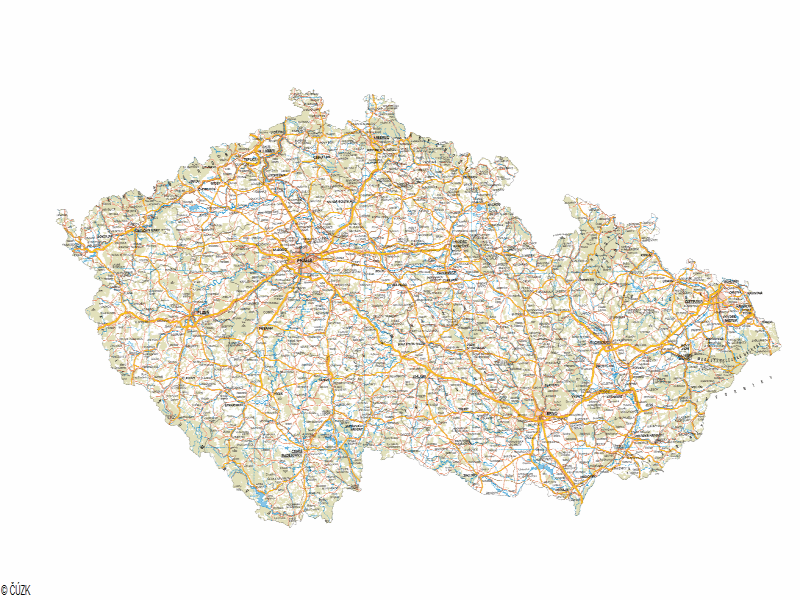
\includegraphics[scale=0.5]{figures/GetMapResponse}


Poslední typ dotazu je volitelný a nazývá se GetFeatureInfo. Ten dotaz, na rozdíl od předchozích, nemusí server podporovat.
Tento dotaz slouží k získán informací o prvcích ve vrstvě. Pokud je v elementu <Layer> uveden argument  queryable 
s hodnotou 1, je možné na tuto vrstvu aplikovat dotaz GetFeatureInfo.  

Jako příklad pro tento typ dotazu je použit WMS server Středočeského kraje. Jedna z WMS služeb, které tento server poskytuje, jsou zóny integrovaného dopravního systému dostupné
na :\url{http://mapy.kr-stredocesky.cz/ids_zony_wms}. 
Nejprve se dotazem GetaCapabilities zjistí informace o WMS serveru a jím poskytovaných datech:

\newcommand{\StredoceskygetCap}{http://mapy.kr-stredocesky.cz/ids_zony_wms?SERVICE=WMS&REQUEST=GetCapabilities}
\begin{alltt}\footnotesize
\href{\StredoceskygetCap}{http://mapy.kr-stredocesky.cz/ids\_zony\_wms?}
\href{\StredoceskygetCap}{SERVICE=WMS\&REQUEST=GetCapabilities\&VERSION=1.3.0}
\end{alltt}

Z odpovědi je patrné, že server obsahuje pouze jednu vrstvu Zony SID, se kterou lze dále pracovat, protože její rodičovská vrstva nemá atribut <Name> nutný pro dotazy GetMap a GetFeatureInfo.

Vrstva je dostupná v jediném souřadnicovém systému. Za povšimnutí stojí opakované uvedení souřadnicové systému a stejného obdélníku BoundingBox v němž jsou poskytována data jak v kmenové vrstvě, tak v jejím potomku Zony SID. Jelikož se tyto elementy vrstvy dědí, stačilo by je uvést pouze v kořenové vrstvě.

Na základě informací z dotazu GetCapabilities byl vytvořen dotaz GetMap: 

\url{http://mapy.kr-stredocesky.cz/ids_zony_wms?SERVICE=WMS&REQUEST=GetMap&VERSION=1.3.0&FORMAT=image/png&LAYERS=sid_zony&CRS=EPSG:2065&BBOX=-834258.9702,-1129697.611,-651189.0329,-968639.3882&WIDTH=1000&HEIGHT=1000}
%% \begin{alltt}\footnotesize
%% \href{\StredoceskygetMap}{http://mapy.kr-stredocesky.cz/ids\_zony\_wms?}
%% \href{\StredoceskygetMap}{SERVICE=WMS\&REQUEST=GetMap\&VERSION=1.3.0\&}
%% \href{\StredoceskygetMap}{&LAYERS=sid_zony\&FORMAT=image/png&CRS=EPSG:2065\&}
%% \href{\StredoceskygetMap}{BBOX=48.093144621684,11.6163532829661,51.4980192528993,19.0628256634265\&}
%% \href{\StredoceskygetMap}{WIDTH=1000\&HEIGHT=1000}
%% \end{alltt}

A výsledný dotaz GetFeatureInfo vypadá takto:
\newcommand{\StredoceskyGetFeatureInfo}{http://mapy.kr-stredocesky.cz/ids_zony_wms?REQUEST=GetFeatureInfo&VERSION=1.3.0&FORMAT=image/png&LAYERS=sid_zony&CRS=EPSG:2065&BBOX=-834258.9702,-1129697.611,-651189.0329,-968639.3882&WIDTH=1000&HEIGHT=1000&INFO_FORMAT=text/html&I=695&J=720&QUERY_LAYERS=sid_zony}
\begin{alltt}\footnotesize
\href{\StredoceskyGetFeatureInfo}{http://mapy.kr-stredocesky.cz/ids\_zony\_wms?}
\href{\StredoceskyGetFeatureInfo}{REQUEST=GetFeatureInfo\&VERSION=1.3.0\&}
\href{\StredoceskyGetFeatureInfo}{FORMAT=image/png\&LAYERS=sid\_zony\&CRS=EPSG:2065\&}
\href{\StredoceskyGetFeatureInfo}{BBOX=-834258.9702,-1129697.611,-651189.0329,-968639.3882\&WIDTH=1000\&HEIGHT=1000\&}
\href{\StredoceskyGetFeatureInfo}{INFO\_FORMAT=text/html\&I=695\&J=720\&QUERY\_LAYERS=sid\_zony}
\end{alltt}


Jak lze vidět, tento dotaz zahrnuje parametry předchozího dotazu GetMap a přidává další:
\begin{itemize}
  \item Parametr REQUEST uvádí typ dotazu GetFeatureInfo 
  \item Parametr INFO\_FORMAT popisuje v MIME tvaru formát odpovědi na tento dotaz. WMS standard neuvádí implicitní formát, který musí server podporovat. V tomto případě se jedná o html soubor. 
  \item Parametry I a J lokalizují prvek, na který dotaz GetFeatureInfo směřuje. Tyto souřadnice reprezentují souřadnicový systém obrázku s jednotkami v pixelech a začátkem v levém horním rohu. Souřadnice os I, J narůstají  
        směrem vpravo resp. dolů. Interval souřadnic je dán parametry WIDTH a HEIGHT, kdy I, J mají rozsah od 0 do WIDTH - 1 resp. od 0 do HEIGHT - 1.  
  \item QUERY\_LAYERS je výčet vrstev, kterých se týká dotaz GetFeatureInfo. 
\end{itemize}

  
\begin{figure}[h!]
 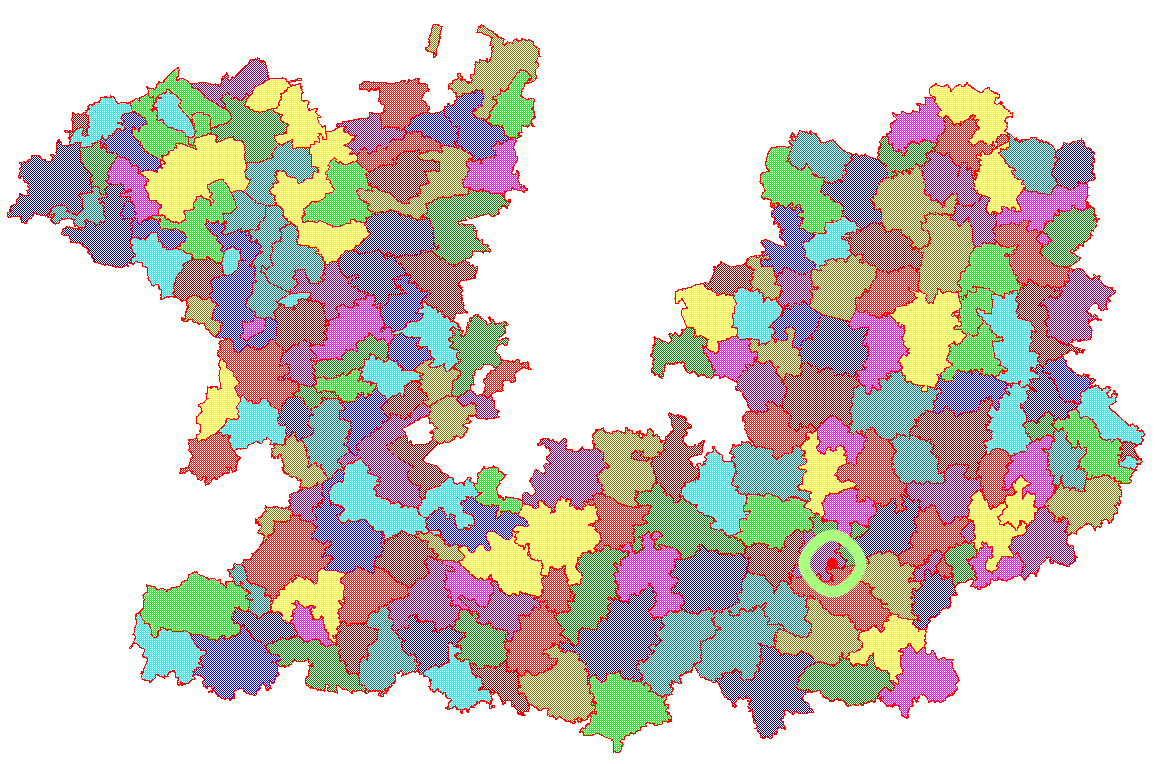
\includegraphics[scale=0.3]{figures/getfeatureinfo}
  \caption{Výsledek GetMap dotazu s bodem o souřadnicích I, J  695 a 720:}
\end{figure}

A jako odpověď server zašle HTML dokument, který se v prohlížeči zobrazí takto:

 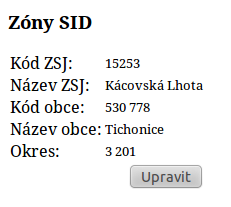
\includegraphics[scale=0.7]{figures/getfeatureinforeply}


Pokud je serveru položen WMS dotaz ve špatném tvaru, vrátí výjimku implicitně ve formátu XML souboru, v němž je blíže specifikována chyba v dotazu. 


\newpage

\section{WMS modul pro GRASS}

Jelikož původně GRASS neměl žádné GUI, jeho moduly jsou přizpůsobeny pro práci v příkazové řádce. Každý modul si lze představit jako funkci, která má definované vstupní argumenty a určené výstupy. Nevýhodou tohoto 
přístupu je, že modul není schopen s uživatelem komunikovat za běhu. Uživatel může jeho chování ovlivnit jen pomocí argumentů, které jsou zadány před spuštěním.

Z tohoto důvodu implementace modulu odpovídá dotazu typu GetMap. Kdy uživatel musí zadat parametry tohoto dotazu a modul se postará a stažení rastru, jeho import do GRASS a případné další úpravy. 


Tento fakt ovšem nebrání úplné interaktivní implementaci podpory WMS do GRASS. Je ji ovšem potřeba rozdělit do dvou částí. První částí je vytvoření WMS modulu, který umožní pracovat s WMS daty i uživatelům, jenž používají
pouze příkazovou řádku.  Do GUI programu je pak možné implementovat interaktivní část.


\subsection{Analýza původního stavu}

 V GRASS GIS již existuje modul r.in.wms umožňující získání WMS dat.
Velkým problémem tohoto modulu je rozdělení jeho kódu do 8 souborů, což jej činí velmi nepřehledným. 
Tento modul byl původně napsán jako shell skript. V GRASS 7 byly všechny moduly v shell skript  přepsány do jazyka Python, což také nepřispělo k jeho zpřehlednění. 

Ještě větším problémem však je, že tento modul selhává při komunikaci s mnoha WMS servery. Z vlastní zkušenosti musím konstatovat, že při používání modul více selhával, než pracoval správně.

Na základě těchto faktů bylo rozhodnuto, že se WMS modul pro GRASS vytvoří od základů znova. Případná oprava chyb ve stávajícím modulu a reorganizace kódu by byla mnohem problematičtější a časově náročnější.

\newpage

\subsection{Stanovení cílů implementace}

Návrh struktury modulu byl realizován na základě těchto požadavků:
\begin{itemize}
  \item Modul bude plně podporovat všechny možnosti dotazu GetMap.
  \item Modul bude komunikovat se serverem prostřednictvím knihovny GDAL\footnote{\url{www.gdal.org/}}  a také pomocí vlastní implementace 
  \item WMS severy mají nastaveny limity pro přenos dat, aby zabránily dotazům, které by je nadměrně zatížily. Tyto limity jsou dány formou maximálních hodnot parametrů WIDTH a HEIGHT dotazu GetMap. 
        Modul bude umět požadavek rozdělit na více WMS dotazů a získat tak požadovaný rastr po částech tzv. dlaždice, které posléze složí do jednoho rastru.
  \item Důležitým prvkem při práci v systému GRASS GIS je lokace. Lokace sdružuje data, která mají stejnou projekci. Její podmnožinou je mapset, který seskupuje data lokace do logických celků. 
        Na začátku práce v GRASS GIS si uživatel vybere lokaci ve které chce pracovat. Následná práce je svázána s touto lokací a jejím souřadnicovým systémem.
 
        Pokud by uživatel chtěl získat rastr z WMS serveru, který neposkytuje data v projekci lokace,  musel by nejprve vytvořit lokaci v projekci WMS dotazu a poté tyto data manuálně transformovat a zkopírovat do pracovní lokace.
	
	Proto bude modul schopen obdržená data automaticky transformovat  do souřadnicového systému lokace, pokud se jejich projekce bude lišit. 
  \item Jelikož existují další rozšíření standardu WMS, jako například Web Map Tile Service \footnote{\url{http://www.opengeospatial.org/standards/wmts}}, struktura modulu umožní snadnou implementaci 
        těchto rozšíření do existujícího kódu. 
  \item Vstupní argumenty modulu budou kompatibilní s modulem r.in.wms. Některé nevýznamné argumenty, které nemají vliv na funkčnost modulu, mohou být vynechány.
  \item Doplňkovou funkcí modulu bude možnost stáhnout a vypsat na standardní výstup obsah Capabilities souboru. Další zpracování toto výstupu bude součástí GUI.  
 \end{itemize}



\subsection{Volba způsobu implemntace}

V GRASS GIS verze 7 mohou být moduly implementovány v jazyce C nebo Python. V jazyce C se implementují moduly, které jsou náročné na výpočetní výkon počítače. 
Rychlost je vykoupena značně delším vývojovým cyklem, neboť programátor je nucen se starat o mnoho věcí, o které se Python postará sám.

Koncepce WMS modulu byla zvolena tak, aby neprováděl žádně složité výpočetní operace, ale aby pro tyto typy operací byly využity již implementované funkcionality 
ostatních GRASS modulů nebo knihoven. Proto byl vybrán jazyk Python. 

Pro práci modulu se staženým rastrem jako je reprojekce a spojení dlaždic byla zvolena knihovna GDAL, která je součástí standardní instalace GRASS.

Tato open source knihovna umožňuje čtení, zápis a reprojekci rastrů.  
Základním prvkem knihovny, který reprezentuje rastrová data je dataset.  Každý dataset reprezentuje rastrová data v určitém formátu, s nimiž pracuje pomocí driveru. Driver je třída, která je schopná číst a zapisovat data v určitém formátu. 

\subsection{Volba vstupních argumentů modulu}


 Vstupních argumenty budou reprezentovat jednotlivé parametry dotazu GetMap. Počet řádků (HEIGHT), sloupců (WIDTH) a geografický rozsah dat (BBOX) 
budou reprezentovány pomocí regionu. 

Region v GRASS je datová struktura, která definuje oblast na základě obdélníku. Tento obdélník je dán mezními kartografickými  souřadnicemi v každé ose a počtem řádků a sloupců pro rastr. Každý region je vztažen k určité projekci, která je totožná s projekcí lokace, ve které je uložen.

Pomocí regionu se určuje rozsah, na kterém bude aplikována činnost modulů.
Oblastí vně regionu nejsou do výpočtů zahrnuty. Vyjímkou jsou moduly, které data načítají jako například modul r.in.gdal. Tyto moduly implicitně načítají data v celém jejich rozsahu, bez ohledu na výpočetní region. 

Vstupní argumenty, které jsou nad rámec parametrů dotazu GetMap, se týkají dlaždicování. Modul umožňuje zadání maximálního počtu řádků 
a slopuců v jednom WMS dotazu. Na základě těchto hodnot se rozdělí získání dat z WMS serveru do několika dotazů a výsledný rastr je složen z rastrů získaných těmito dotazy. 
   


\subsection{Implementace modulu}

TODO UML Diagram

Třída WMSBase je abstraktní třída, která vykonává ty funkce, které se netýkají komunikace s WMS serverem. Tato komunikace je implementována v odvozených WMSGDALDrv a WMSDrv.

\subsubsection{Třída WMSBase}


Hlavními funkcemi třídy WMSBase je výpočet parametrů pro komunikaci s WMS serverem, import již stažených dat do lokace a dodatečné úpravy těchto dat pomocí modulů GRASS. 

Tato třída obsahuje tyto důležité metody:  
\begin{itemize}
  \item \_GetCapabilities - Vytvoří a pošle WMS serveru dotaz typu GetCapabilities, následně obdrženou odpověď vypíše na standardní výstup a tímto se běh modulu ukončí. 
  \item \_GetMap - Tato metoda postupně volá níže zmíněné metody v pořadí v jakém jsou vedeny. 
  \item \_initializeParameters - Metoda inicializuje proměnné potřebné pro další běh modulu. Jde o uložení hodnot ze slovníků vstupních argumentů do separátních proměnných a také získání hodnot ze zvoleného regionu.
  \item \_computeBbox - Pokud se liší projekce, ve které budou data staženy z WMS serveru a projekce pracovní lokace, je potřeba souřadnice, které vymezují region transformovat do projekce WMS dotazu, aby bylo možně definovat parametr BBOX ve správném souřadnicovém systému.

                        Zpravidla výsledkem transformace není obdélník se stranami rovnoběžnými se souřadnicovými osami systému, ale obecný čtyřúhelník. Protože parametr BBOX WMS dotazu GetMap  musí být uveden  v tomto obdélníku, jsou vybrány extrémní souřadnice, které tvoří obdélník rovnoběžný s osami souřadnicového systému.      
  \item \_download - Jedná se o metodu virtuální, definovanou v potomcích třídy, která dotazem GetMap stáhne rastr a uloží jej do dočasného souboru. Zpravidla jsou rastrová data poskytovaná WMS serverem tříkanálová reprezentující RGB systém barev. Pokud jde o rastr s průhlednými plochami, obsahuje ještě alfa kanál, který definuje průhlednost pixelů. Návratovou hodnotou metody je cesta k souboru s rastrem.
  \item \_createOutputMap - Pokud je to potřeba, tato metoda nejprve pomocí utility gdalwarp knihovny GDAL transformuje rastr do projekce lokace. Transformovaný rastr je uložen do nového souboru. 
                            Jelikož rastr je matice o určitých počtech sloupců a řádků, čemuž ale tvar transformovaného rastru zpravidla již neodpovídá, je potřeba mít informaci o tom, který pixel odpovídá původnímu rastru 
                            a který pixel již nereprezentuje data původního rastru. Tato informace je zahrnuta do alfa kanálu. Pixely, které do původnímu rastru nepatří mají hodnotu v alfa kanálu plně průhledného pixelu.  Pokud transformovaný rastr neobsahuje alfa kanál, utilita gdalwarp\footnote{\url{http://www.gdal.org/gdalwarp.html}} jej přidá.
\end{itemize}

Posléze pomocí modulu r.in.gdal\footnote{\url{http://grass.fbk.eu/gdp/html_grass64/r.in.gdal.html}} importuje rastrová data do pracovní lokace.
Modul vytvoří v pracovní lokaci rastrové vrstvy odpovídající jednotlivým kanálům importovaného rastru. Tyto vrstvy jsou pomocí modulu  r.composite\footnote{\url{http://grass.fbk.eu/gdp/html_grass64/r.composite.html}} sloučeny do jedné barevné vrstvy. 

Aby byly správně interpretovány průhledné plochy výsledné rastrové vrstvy, před spuštěním modulu r.composite, se vytvoří z alfa kanálu inverzní maska. Maska se v GRASS používá v těch případech, kdy rozsah dat, nad nimiž bude modul pracovat, nelze vyjádřit pomocí regionu. Maska je v GRASS reprezentována rastrovou vrstvou, jejíž název je MASK. Pixely, kde je maska definována nejsou brány při výpočtu v úvahu. 

Při použití masky vytvoří modul r.composite barevný rastr i s průhlednými pixely definovanými v alfa kanálu.

Modul za svého běhu vytvoří několik dočasných souborů. Tyto dočasné soubory jsou smazány ihned poté, co již nejsou potřeba. Pokud však uživatel neočekávaně přeruší běh programu, může se stát, že některý soubor nebude smazán. Aby se tomuto zabránilo,
je v destruktoru třídy, který se volá i při neočekávaném ukončení modulu, provedeno smazání těchto souborů, pokud nebyly odstraněny. Toto je provedeno i s vrstvami, které reprezentují jednotlivé barevné kanály a maskou. 





\subsubsection{Třída WMSGDALDrv}

Tato třída přistupuje k datům WMS serveru prostřednictvím WMS driveru knihovny GDAL. Parametry WMS dotazu jsou driveru předány ve formě XML souboru \footnote{\url{http://www.gdal.org/frmt_wms.html}}. 
Driver následně stáhne data a uloží je do souboru ve formátu GeoTiff. 



\subsubsection{Třída WMSDrv}

Tato třída komunikuje se serverem přímo, bez použití další knihovny. Nejprve je ze vstupních parametrů vytvořen WMS dotaz. 
Pak následuje výpočet rozměrů dlaždic v souřadnicovém systému projekce, rozměru dlaždic v pixelech a jejich počet. Na základě těchto hodnot jsou v cyklu staženy jednotlivé dlaždice, kdy je k WMS dotazu přidán parametr BBOX pro konkrétní dlaždici, tento dotaz je poslán WMS serveru a do dočasného souboru je uložen stažený rastr. Spojování dlaždic do jednoho rastru je řešeno pomocí knihovny GDAL. Při prvním průchodu cyklu se vytvoří nový dataset, kde se dlaždice postupně, tak jak jsou stahovány, spojují. 

\subsection{Zajímavé problémy a jejich řešení}

Při implementaci třídy WMSDrv se vyskytl problém při dlaždicování.
Při stažení barevného jednokanálového rastru (např. PNG, GIF) s přiloženou globální tabulkou barev vznikl po spojení jednotlivých dlaždic rastr, který tuto tabulku neobsahoval.

Protože v tomto případě konkrétní barvy jednotlivých kanálů jsou definovány až v tabulce barev, není možné bez této tabulky správně interpretovat hodnoty pixelů, které  zde představují pouze odkazy na položky tabulky. V různých dlaždicích jsou stejné barvy definovány jinými položkami tabulky barev a hodnota pixelů na ně odkazující se v nich liší. 
Při spojování dlaždic knihovna GDAL nebrala tabulku barev v úvahu a interpretovala přímo hodnoty těchto pixelů. Výsledný rastr se spojenými dlaždicemi vypadal například takto: 

 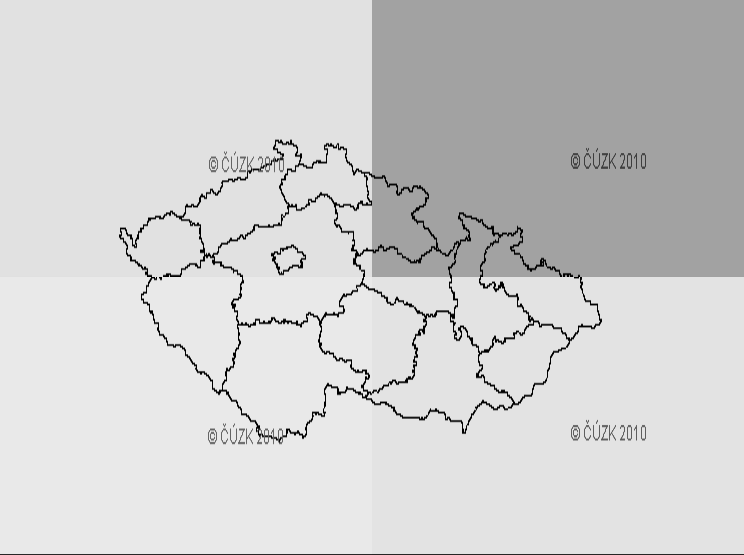
\includegraphics[scale=0.4]{figures/color_table_problem.png}



Tento problém byl vyřešen pomocí upraveného kódu GDAL utility pct2rgb \footnote{\url{www.gdal.org/pct2rgb.html}}. Tento kód obsahuje metoda \_pct2rgb třídy  WMSGDALDrv.
Tato metoda vytvoří 4 kanálový dataset (RGB + alfa vrstva), a do jednotlivých kanálů jsou pixel po pixelu přiřazovány jejich hodnoty z tabulky barev. 

\subsection{Ukázka práce modulu}

Nyní je modul dostupný pod názvem r.in.wms2 v repozitáři GRASS AddOns \footnote{\url{http://svn.osgeo.org/grass/grass-addons/}}. V tomto repozitáři jsou uloženy nové funkcionality implementované do GRASS, které je ještě potřeba otestovat uživateli a dokončit jejich vývoj. Až potom je možné tyto funkcionality  začlenit přímo do programu. 


Modul se do GRASS z repozitáře nainstaluje pomocí tohoto příkazu:
\begin{alltt}\footnotesize
g.extension extension=r.in.wms2
\end{alltt}

\subsubsection{Vstupní argumenty}

V GRASS GIS mají moduly dva typy vstupních argumentů. Argumenty, které nesou binární informaci 0/1 jsou modulu předány ve formě tzv. flags, což řetězce uvedené za pomlčkou. Pokud je tento flag uveden mezi argumenty při spuštění modulu, nese hodnotu 1, pokud však uveden není, je mu přiřazena hodnota 0. 

\begin{table}[h]
\centering
\begin{tabular}{|c|l|}      \hline
  Flag      &    Popis				\\ \hline
   -o        &  Data nebudou obsahovat průhlednou  vrstvu.\\ \hline
   -c       &  Vypíše na výstup Capabilities soubor.\\ \hline
   -d       &  Nepoužije knihovnu GDAL pro komunikaci s WMS serverem, ale vlastní řešení. \\ \hline
\end{tabular}
\caption{Flagy modulu r.in.wms2}
\label{tab:flagy}
\end{table}

Dalším typem vstupních argumentů je parametr. Parametr obsahuje jako hodnoty textové řetězce. I v případě, že argument obsahuje číselnou hodnotu, je tato hodnota uložena jako text a modul ji posléze musí převést na číselný typ. 

Vstupní parametry modulu jsou:
\begin{itemize}
  \item   output -  Povinný parametr. Název vrstvy vytvořené modulem v lokaci.
  \item   mapserver -  Povinný parametr. URL adresa WMS serveru.
 \item     layers - Povinný parametr. Uvádí se ve stejném formátu jako v getMap parametru LAYERS.
 \item     srs - Číslo EPSG kódu, který definuje projekci WMS dotazu. 
 \item     region - Název regionu. Pokud není uveden, je použit aktuálně nastavený region. 
 \item     wms\_version - Verze WMS protokolu, lze uvést 1.1.1\ (implicitní) nebo 1.3.0 
 \item     format - Formát rastru WMS dotazu. Možné hodnoty jsou  geotiff (implicitní), tiff, jpeg, gif, png. 
 \item     method - Pokud projekce rastru z WMS dotazu a projekce lokace nejsou stejné, tento parametr definuje jakou metodou bude rastr transformován do projekce lokace. Může mít tyto hodnoty: near (implicitní), bilinear, cubic, cubicspline.

 \item    maxrows - Číslo, které definuje maximální počet pixelů v řádce jedné dlaždice. Implicitně 400.
 \item    maxcols - Číslo, které definuje maximální počet pixelů ve sloupci jedné dlaždice. Implicitně 300.
 \item    urlparams - Zde lze uvést další parametry WMS dotazu GetMap.
 \item    styles - Styly vrstev ve stejném formátu jako v getMap parametru STYLES.
 \item    bgcolor - Pokud je v dotazu uvedený flag -o, všechny plochy které by byly průhledné, budou vyjádřeny barvou uvedené v tomto parametru. Barva se uvádí v hexadecimálním RGB formátu. Implicitní je bílá barva (0xFFFFFF
).
\end{itemize}

\subsubsection{Příklad}

Pro příklad bude použit WMS server\footnote{\url{http://iceds.ge.ucl.ac.uk/cgi-bin/icedswms}} poskytující družicová data. Na zíkladě informací získaných pomocí GetCapabilities dotazu, je možné spustit modul například s těmito parametry:

\begin{alltt}\footnotesize
r.in.wms2 -d mapserver=http://iceds.ge.ucl.ac.uk/cgi-bin/icedswms \\ layers=bluemarble,landsat\_1\_01 styles=default,default
output=landsat srs=4326 format=png maxcols=500 maxrows=600
\end{alltt}

Při spuštění modulu byla projekce lokace totožná s projekci rastru z WMS dotazu (EPSG:4326). Region byl dán obdélníkem o geografických souřadnicích -20° z. d., 30° s. š., 40° v. d., 65° s. š. a počet pixelů v řádcích byl 700 a  ve sloupcích 1200. Protože byl počet pixelů v obou dimenzích větší než parametry maxcols a maxrows, muselo být stažení rastru rozděleno na stažení 4 dlaždic, které byly následně spojeny.

Pro práci s regiony je určen modul g.region. Pomocí tohoto modulu je možné modifikovat parametry regionů, vytvářet nové, nebo zjišťovat hodnoty parametrů regionů.

Takto vypadá stažený rastr:

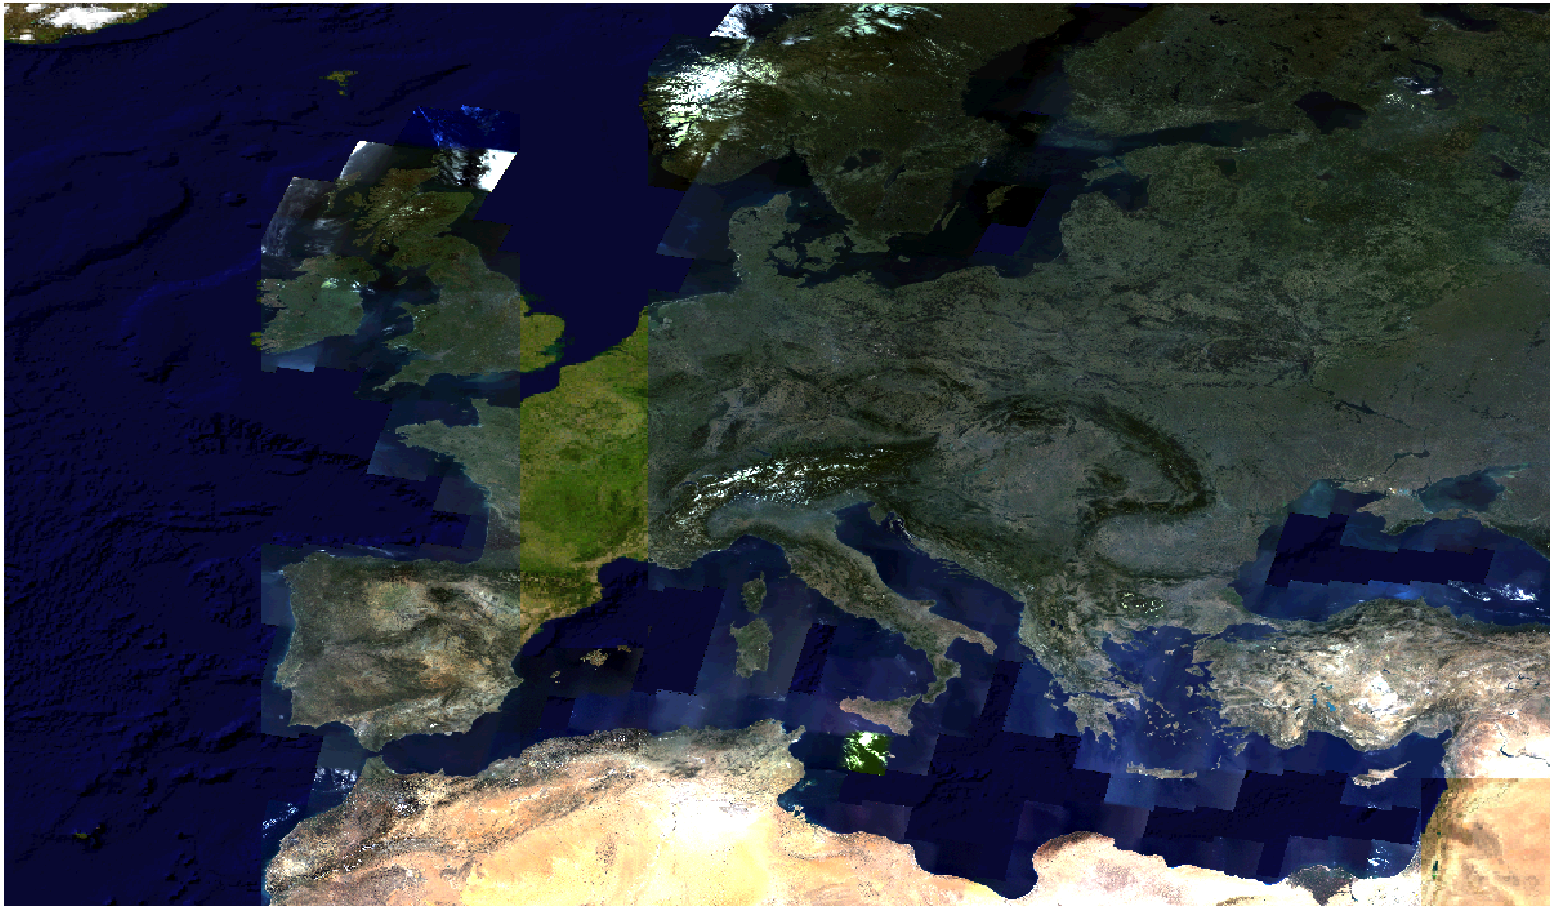
\includegraphics[scale=0.28]{figures/GRASS_WMS_obrazek.png}


\subsection{Další vývoj}

Po otestování uživateli by se měl modul r.in.wms2 stát součástí GRASS a nahradit modul r.in.wms. Pokud k tomu dojde bude pravděpodobně přejmenován na r.in.wms. 

Tento modul je pouze základní částí integrace WMS do GRASS GIS. Nyní je dalším krokem vytvořit interaktivní WMS řešení v GRASS GIS, které by se uživatelskou přívětivostí přiblížilo programům  ArcGis(\url{http://www.arcgis.com/}) nebo QGi(\url{http://www.qgis.org/}). Tyto programy mají z uživatelského pohledu velmi dobbrou podporu WMS. 

Idea tohoto řešení je, že uživatel si na základě dialogu vygenerovaného z Capabilities souboru vybere data která chce zobrazit a v GRASS GUI se přidá nová WMS vrstva. Tato vrstva bude dynamicky získávat data, v závislosti na aktuálním rozsahu mapového okna. 

V GRASS GIS 7 již existuje dialogové okno, které na základě vložené URL adresy stáhne Capabilities soubor a z tohoto souboru zobrazí dostupné vrstvy. 

Tento dialog funguje tak, že po zadání URL adresy se zavolá modul r.in.wms s flagem -l, a ten na standardní výstup vypíše seznam vrstev z Capability souboru. Tyto vrstvy jsou pak zobrazeny v dialogovém okně.

Aby tento dialog umožnil uživateli využít všech možností WMS serveru, nestačí jen vypsat seznam vrstev, ale je také potřeba zobrazit k výběru dostupné formáty, projekce uživatelem vybraných vrstev a také třeba metadata s informacemi o vrstvách. K tomu nestačí jen prostý výpis seznamu vrstev, ale je potřeba pracovat s celým obsahem Capabilities souboru. 

V rámci bakalářské práce, byly již učiněny některé kroky, k vylepšení tohoto dialogu. 

Dialog nyní využívá modul r.in.wms2, který umožňuje vypsat celý obsah Capabilities souboru na standardní výstup. Tento výstup je načten a posléze zpracován do takové datové struktury, která ke každé vrstvě umožňuje zjistit seznam elementů  včetně těch děděných, což je největší problém při zpracování Capabilities souboru. Na základě této struktury lze v dialogu zobrazit strom  vrstev, který odráží uspořádání elementů <Layer> v Capabilities souboru. 

Také tento dialog byl rozšířen o pole, ve kterém se vypisují metadata o vrstvách, kliknutím na jednotlivé položky stromu vrstev. 

Nyní je potřeba zobrazit všechny potřebná data v tomto dialogu.

 Dalším krokem bude v GUI vytvořit rastrovou WMS vrstvu, která, pokud bude zobrazena v mapovém okně, spustí na pozadí modul r.in.wms. Tento modul bude spouštěn s parametry, které budou zadány v dialogovém okně před přidáním vrstvy. Při každém volání z mapového okna se změní pouze parametr region, který bude odpovídat aktuálnímu rozsahu a rozlišení pixelu  mapového okna.
 
Při pohybu mapového okna se mění pouze rozsah, ze kterého se zobrazují data. Často se stává, že uživatel pohne s oknem jen o kousek, kdy značná část okna je pořád v rozsahu již stažených dat. Proto by bylo možné toto optimalizovat tak, že by došlo ke stažení jen těch dat, která v pohledu chybějí a nemusela by se stahovat data v celém rozsahu mapového okna.


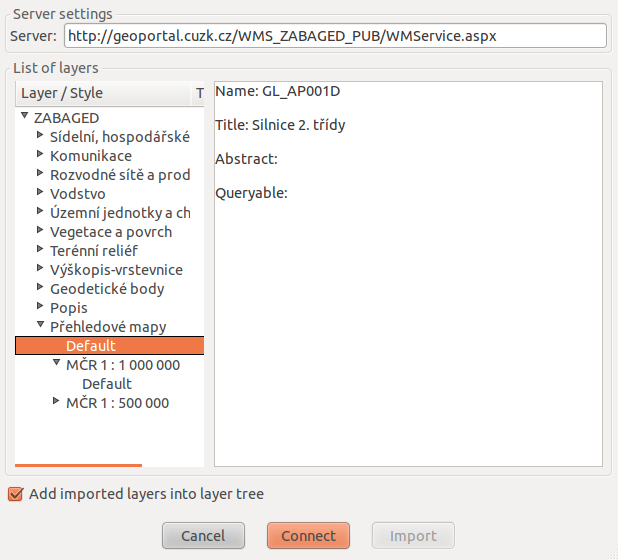
\includegraphics[scale=0.5]{figures/GRASS_dialog_soucasny_stav.png}

\newpage

\section{ WMS modul pro SAGA GIS}

V SAGA GIS je koncept modulu odlišný od GRASS GIS. Jedním z důvodů tohoto rozdílu může být to, že SAGA je software mnohem mladší než GRASS, proto v době, kdy byl jeho vývoj započat, bylo grafické rozhraní programů již standardem, na rozdíl 
 od počátku vývoje GRASS GIS. 

Proto moduly SAGA GIS mohou být více interaktivní a za běhu komunikovat s uživatelem, čehož lze využít při vývoji WMS modulu.

\subsection{Analýza původního stavu}

Do aktuální verze (2.0.8) SAGA GIS byla nově začleněna experimentální knihovna Garden - Web Service Data Access. Tato knihovna obsahuje modul Import a Map via Web Map Service (WMS), který umožňuje získat data z WMS serveru.
Modul funguje tak, že po spuštění vytvoří ze zadané URL adresy dotaz GetCapabilities, na základě odpovědi vytvoří dialog, ve kterém uživatel může vybrat parametry pro získání rastru z WMS serveru. 

Tento koncept modulu je uživatelsky velmi přívětivý, jelikož stačí znát pouze URL adresu a o vše ostatní se postará modul. Uživatel si pak vybere z možností, které server nabízí a nemusí tyto informace zjišťovat jiným způsobem. 


Jelikož se jedná o experimentální modul, obsahuje velké množství nedostatků. Zejména tyto:

\begin{itemize}
\item Nesprávně zpracovává Capabilities soubor, a proto vygeneruje dialog, který nedovoluje uživateli vybrat si ze všech možností, jenž server nabízí. Omezení dialogu jsou tato:
\begin{itemize}
 \item     V dialogu nenabídne všechny vrstvy, ale pouze ty, které jsou přímými potomky kořenové vrstvy, což je výrazné omezení, jelikož se týká přímo poskytovaných dat WMS serveru.
 \item 	   Nelze určit pořadí vrstev, v jakém budou  zobrazeny na výsledné mapě.
 \item 	   Neumožňuje výběr stylu vrstvy .
 \item 	   Při načítání vrstev nebere v úvahu dědičnost	  . 
\end{itemize}
\item Nepodporuje dlaždicování. 
\end{itemize}


 
\subsection{Stanovení cílů implementace}


Základní koncept modulu bude stejný jako u modulu experimentálního. To znamená, že modul nejprve získá Capabilites soubor z WMS serveru, vygeneruje pro něj nabídku a na základě zvolených hodnot pomocí 
dotazu GetMap stáhne požadovaný mapový rastr a naimportuje jej do programu. 

Při implementaci by měly být naplněny tyto cíle:
\begin{itemize}
\item  Modul bude schopen správně schopen zpracovat Capabilities soubor ve standardu 1.1.1 a 1.3.0.  Jelikož ne všechny WMS servery plně podporují WMS standardy, bude napsán tak, aby si poradil s těmi prohřešky proti standardu, které jsou nejčastější, jako je například neuvedení informace o stylech vrstvy.  
\item Nabídka parametrů umožní uživateli využití všech možností WMS dotazu GetMap.
\item Modul bude schopen transformovat rastr do uživatelem požadováného zobrazení. V SAGA GIS neexistuje ekvivalent lokace jako v GRASS GIS. Z vrstvami lze pracovat v libovolném zobrazení najednou. Existuje i modul,
      který umí transformovat rastr do jiné projekce. Tato funkcionalita ulehčí uživateli práci, protože často se stává že WMS server neposkytuje data v uživatelem požadované projekci. 
Také modul umožní zadat hodnotu parametru BBOX v souřadnicích požadované projekce a za běhu modulu, tyto souřadnice transformovat do projekce WMS dotazu.
\item Umožní implementovat další rozšíření WMS standardu. 
\end{itemize}


\subsection{Volba způsobu implementace}

Modul byl implementován v jazyce C++, ve kterém je napsán celý program SAGA a všechny jeho moduly.  Byla snaha využít objektových rysů jazyka C++, které mohou ulehčit budoucí rozšiřování 
modulu o podporu dalších nástaveb WMS a celkově pomoci vytvořit čitelnější kód. 

Další důležitou volbou, před vlastní implementací modulu, bylo rozhodnutí, zda v tomto modulu spouštět další SAGA moduly, které  by například transformovaly rastr do požadované projekce nebo transformovaly souřadnice. 

Nakonec bylo rozhodnuto tyto operace provést před importem do SAGA GIS pomocí knihovny GDAL (reprojekce) a knihovny PROJ4 (transformace souřadnic), jelikož spouštění ostatních modulů z modulu není v SAGA GIS tak jednoduché jako v GRASS, kde je možné modul zavolat prostřednictvím jediné funkce. 

\subsubsection{Knihovna PROJ4}

Knihovna PROJ4 \url{http://trac.osgeo.org/proj/} je open source projekt, který dovoluje transformovat souřadnice do různých projekcí, které jsou součástí této knihovny.Také umožňuje definovat vlastní 
projekce. Tuto knihovnu používá např. GRASS GIS, SAGA GIS nebo GDAL.

\subsection{Moduly v SAGA GIS}

Každý modul v SAGA GIS je potomkem třídy CSG\_Modul. Vstupní argumenty modulu, které se zadávají před spuštěním jsou uvedeny v konstruktoru třídy modulu.

Argumenty jsou prvky instance třídy CSG\_Parameters Parameters. 
Metoda OnExecute je další metoda, kterou musí každý modul obsahovat. Tato metoda je volána při spuštění modulu. 

V SAGA GIS existují ještě interaktivní moduly, které jsou schopny reagovat např. na kliky v mapovém okně nebo na stisky kláves a jejich struktura se liší.    


\subsection{Implemntace modulu}
Modul je implementován jako přímý potomek třídy CSG\_Module. Tato třída se nazývá CWMS\_Import a má na starosti všechny funkce, které jsou přímo spojeny s programem SAGA GIS.

Jedná se o vytvoření dialogů na základě Capabilities souboru, který je stažen a načten  skrz členy třídy CWMS\_Base a o import rastru do programu. 

\subsubsection{Třída CWMS\_Base}

Tato třída nejprve pomocí instance CWMS\_Capabilities, získá Capabilities data z WMS serveru. Na základě těchto dat třída CWMS\_Import vygeneruje dvě nabídky, ze kterých uživatel vybere parametry dotazu GetMap. 

Potom je spuštěna metoda GetMap, která stáhne a transformuje rastr do požadované projekce. Tato metoda vrátí cestu k souboru, ve kterém je uložena již výsledná rastrová mapa určená k načtení do programu.
Struktura a funkce této metody jsou velmi podobné WMS modulu pro GRASS. Největším rozdílem je to, že nenačítá výslednou mapu do programu, protože k tomu je potřeba využít neveřejných členů třídy CSG\_Module, 
které nejsou z této třídy dostupné. Toto by šlo obejít deklarováním CWMS\_Base přítelem CWMS\_Import, což je potomek CSG\_Module. Tato deklarace však porušuje zapouzdřenost, jeden za základních principů objektově orientovaného
programování. Proto je metoda \_Import\_Map součástí třídy CWMS\_Import, z níž může přistupovat k těmto členům.

Metoda GetMap volá tři neveřejné metody v tomto pořadí:
\begin{itemize}
 \item \_ComputeBbox - Transformuje souřadnice obdélníku, pokud jsou zadány v jiné projekci než, kterou nabízí WMS server. Transformace je provedena pomocí knihovny PROJ4, která je standardně přítomna v každé SAGA instalaci. Z transformovaných bodů jsou vybrány extrémní souřadnice, které pak definují parametr BBOX WNS dotazu. 
 \item \_Download - Tato metoda je virtuální a je pouze v této třídě deklarovaná. 
 Návratovou hodnotou této metody je casta ke souboru rastru, ve kterém jsou již spojeny dlaždice z jednotlivých WMS dotazů.
 \item \_GdalWarp - Tato metoda pomocí knihovny GDAL, pokud je to potřeba, transformuje stažený rastr, do výsledné projekce. Jedná se o modifikovaný kód z \url{http://www.gdal.org/warptut.html}.
\end{itemize}

\subsubsection{Třída CWMS\_Gdal\_drv}

Členění této třídy a funkce jejich metod jsou v zásadě stejné jako u třídy WMSGDALDrv v GRASS modulu. Metoda \_CreateGdalDrvXml vytoří XML soubor s parametry pro GDAL WMS driver, 
který metoda  \_Download použije pro stažení rastru z WMS serveru. 


\subsubsection{Třída CWMS\_Capabilities}

Tato  třída pomocí metody Create, jejíž argumentem je URL adresa WMS serveru, vytvoří WMS dotaz GetCapabilities a následně načte do své struktury XML soubor s odpovědi.

K načtení XML souboru jsou použity třídy knihovny WxWidgets, která je součástí programu SAGA. Pomocí třidy wxXmlDocument této knihovny je načten XML soubor a vytvořena datová struktura reprezentující XML strom. Ekvivalentem XML elementu v této struktuře je třída wxXmlNode, která obsahuje odkaz na rodiče a na své přímé potomky. 

Pokud by neexistovala dědičnost ve stromu elementů <Layer>, bylo by možné snadno zjistit všechny informace o vrstvě z jejího wxXmlNode a stačilo by pouze uchovat ve třídě CWMS\_Capabilities odkaz na kořenový element XML souboru. Protože však tato dědičnost existuje, bylo potřeba nějakým způsobem ke každé vrstvě seskupit všechny její elementy, včetně zděděných. 
  

Proto byla vytvořena třída  CWMS\_Layer, která obsahuje ukazatel na rodičovskou vrstvu a na její přímé potomky ve stromu. Důležitým členem třídy je kontejner map s názvem m\_LayerElms, který obsahuje položky, mající jako klíč název elementu, který je přímým potomkem elementu <Layer> a vektor ukazatelů na objekty wxXmlNode reprezentující tyto elementy. Tento kontejner zahrnuje všechny elementy, včetně elementů získaných dědičností. Jelikož se jedná o ukazatele na objekty, nejsou ukládány duplicitní informace, ale všechny vrstvy, které dědí stejný element odkazují na tentýž objekt. 

Toto uspořádání je vytvořeno rekurzivně, kdy je strom elementů <Layer> procházen od kořene k jeho listům. Po vytvoření instance  CWMS\_Layer je zavolána její metoda Create, která z kontejneru m\_LayerElms  rodičovského objektu třídy CWMS\_Layer, který je již díky rekurzi vytvořen, vybere ty objekty, které dědí a naplní vlastní kontejner m\_LayerElms. Aby kontejner obsahoval všechny přímé potomky elementu <Layer>, jsou potom přidány elementy, které se nedědí. 

\subsection{Ukázka práce modulu}

Pokud je modul načten do SAGA GIS je dostupný v knihovně modulů Web Service Data Access pod názvem WMS. Po otevření modulu se objeví toto dialogové okno:

 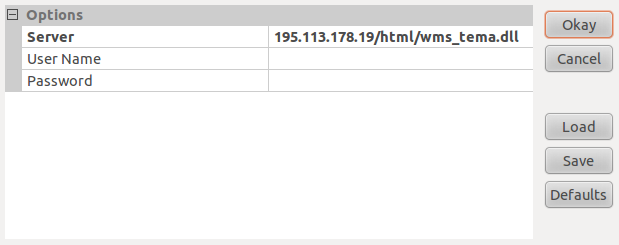
\includegraphics[scale=0.4]{figures/SAGA_okno1.png}

V tomto případě byla jako URL adresa zadán WMS server Pardubického kraje. 
Pokud server vyžaduje uživatelské jméno a heslo, lze tyto parametry zadat do polí User Name resp. Password. 

Jako další dialog se zobrazí strom vrstev. které server poskytuje:

 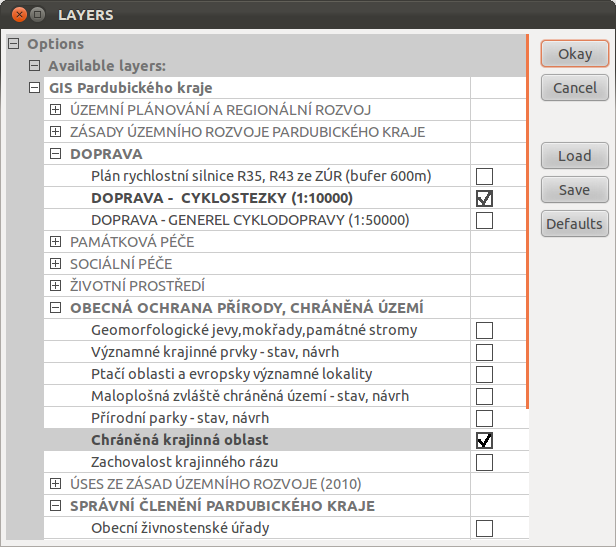
\includegraphics[scale=0.6]{figures/SAGA_okno2.png}
 
Je možné vybrat pouze ty vrstvy, které mají definován uveden element <Title>. Jak bylo již výše zmíněno, vrstvy které tento element postrádají nelze použít pro dotaz typu GetMap. 
 
 
 Posledním dialogem generovaným modulem je nastavení parametrů WMS dotazu. 
Pro tento příklad, kdy byly vybrány vrstvy Obce s rozšířenou působností, Hranice obcí, DOPRAVA - CYKLOSTEZKY (1:0000) a Chráněná krajinná oblast vypadá takto:
 
  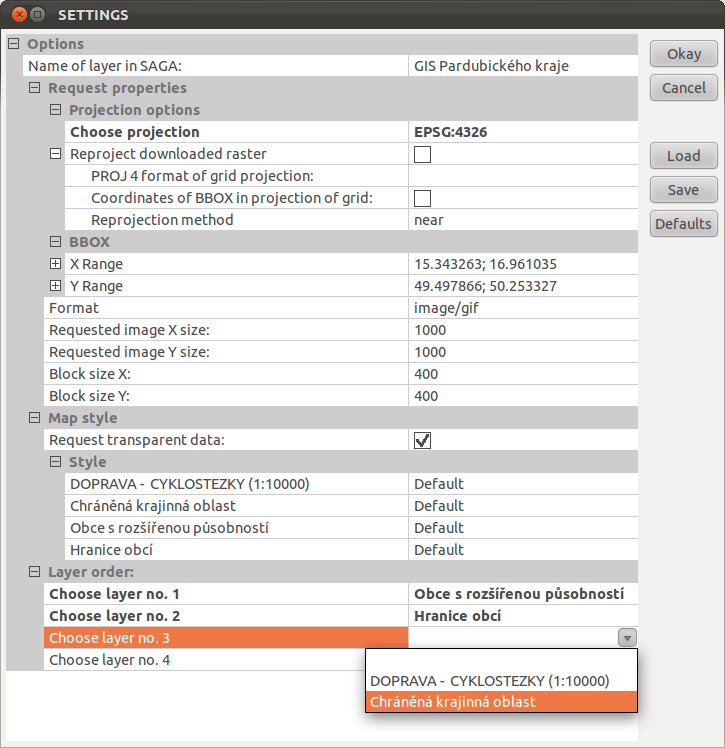
\includegraphics[scale=0.6]{figures/SAGA_okno3.png}

Dialog obsahuje tyto položky:

\begin{itemize}
\item Name of layer in SAGA: Představuje název vrstvy v SAGA se staženými rastrem.
\item Choose projection: Tato nabídka obsahuje seznam všech společných projekcí, ve kterých jsou dostupné vybrané WMS vrstvy. Pokud se změní projekce, jsou automaticky změněny hodnoty v oddíle BBOX, na hodnoty pro tuto projekci. Toto slouží k usnadnění orientace uživatele, v jakém rozsahu jsou data poskytována. 
\item Pokud uživatel chce vrstvu transformovat do jiné projekce, definuje ji v parametru PROJ4 format of grid projection. Pokud má být rastr transformován, musí rovněž být zatržena volba Reproject downloaded raster. Jestliže jsou zadány souřadnice BBOX v projekci, do které rastr bude transformován, je potřeba zatrhnout volbu Coordinates of BBOX in projection of grid. 
\item Za oddílem BBOX jsou definovány rozměry staženého rastru v pixelech (Requested image X/Y size)a počet pixelů v řádcích a sloupcích jedné dlaždice (Block size X/Y). 
\item V oddíle Map Style volba Request transparent data udává, zda mají být požadovány data s průhlednou vrstvou-. 
V pododdíle Style jsou zobrazeny nabídky se všemi dostupnými styly jednotlivých vrstev.  

\item V posledním oddíle je možné určit pořadí vrstev, v jakém budou budou vykresleny ve výsledné mapě. Aby si uživatel nemusel pamatovat, které vrstvy již vybral ve výše uvedených nabídkách, jsou již vybrané vrstvy z těchto nabídek odstraněny.  Výběr pořadí vrstev by bylo lepší implementovat jako seznam položek, které by šlo přesouvat. Avšak SAGA API neumožňuje vytvořit takovýto prvek v dialogu modulu, proto byl vytvořen tento systém nabídek.

WMS server v tomto příkladě nepodporuje standard zcela správně. Problémem je, že vrstvy řadí v opačném pořadí, takže ta, která je vybraná jako první (Obce s rozšířenou působností), bude překryta ostatními vrstvami. Pokud by se WMS server choval správně, měla by být zobrazena nad všemi vrstvami. 
\end{itemize}

Následně na základě zvolených parametrů modul stáhne data z WMS serveru a importuje je do SAGA GIS. V tomto případě stažená data vypadají takto:

 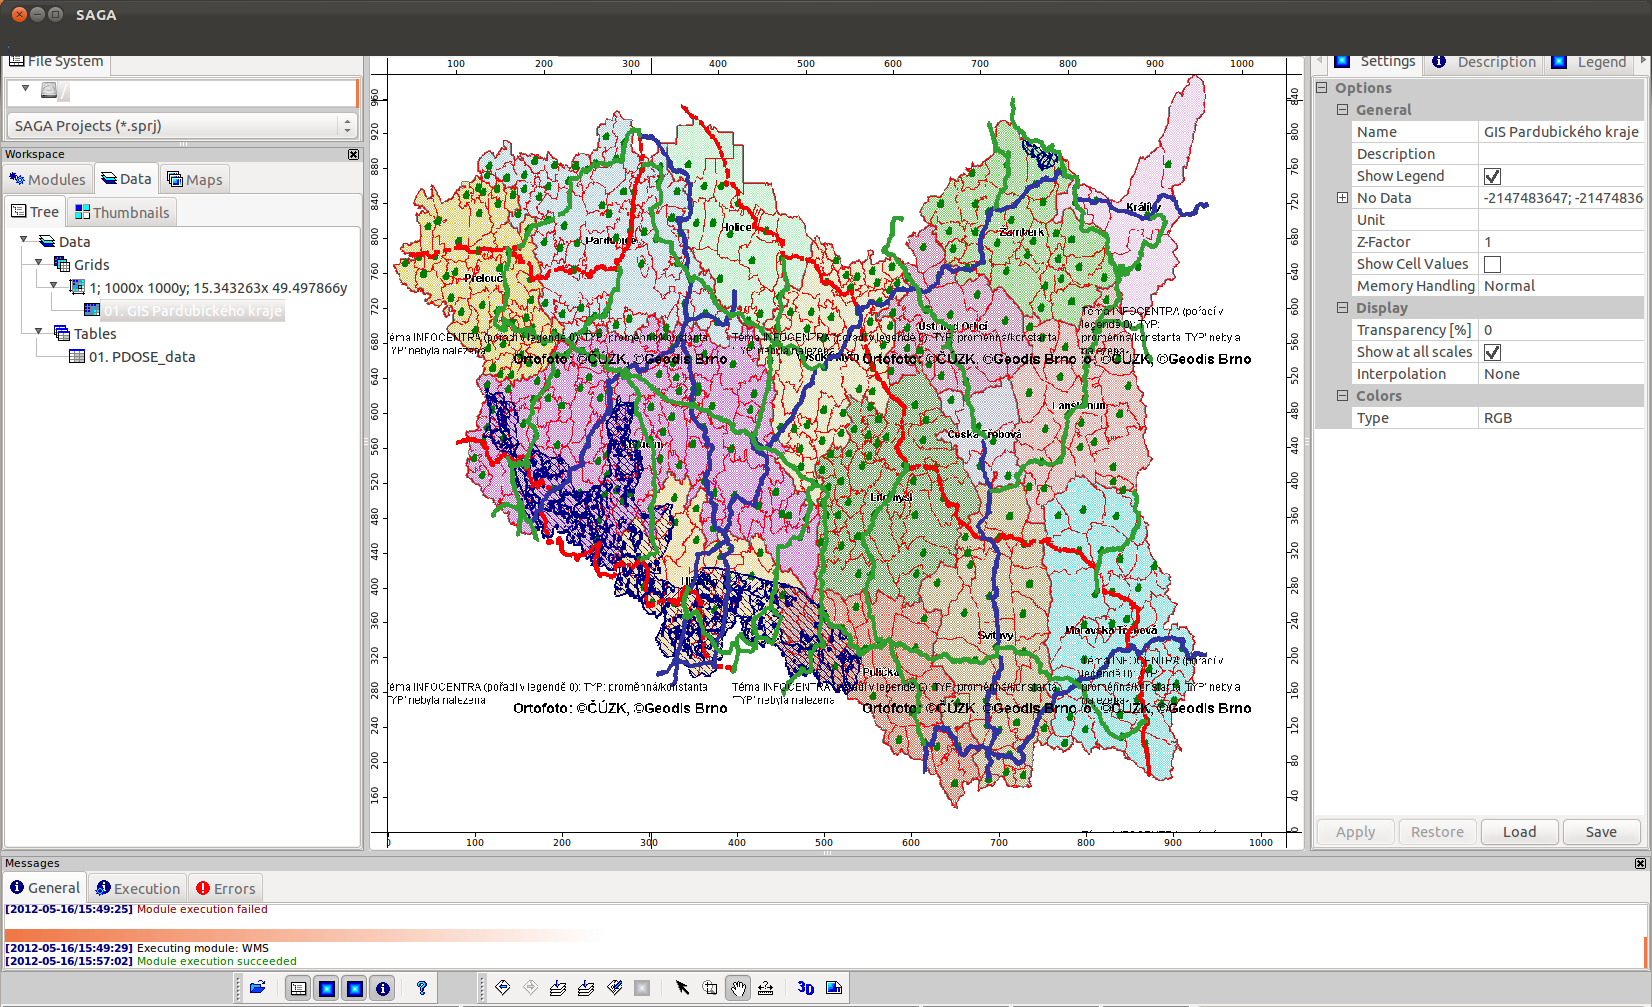
\includegraphics[scale=0.25]{figures/SAGA_okno4.png}
\subsection{Další vývoj}

Nejdůležitějším krokem, který by se měl udát v blízké době, bude zveřejnění zdrojových kódů modulu komunitě uživatelů SAGA, aby bylo možné modul řádně otestovat a upravit jej podle připomínek uživatelů. Způsob zveřejnění bude muset být ještě dohodnut s vývojáři SAGA.

Do modulu by měla být přidána nová třída CWMS\_drv, která bude přímo implementovat komunikaci s WMS serverem. Princip této implementace bude velmi podobný třídě WMSDrv v modulu GRASS. Neměl by být problém začlenit tuto třídu do stávajícího kódu, protože stávající struktura modulu je již k tomu přizpůsobena.

Dalším krokem by bylo provázání modulu s mapovým oknem, kdy by docházelo k stahování dat na základě rozsahu okna. 

K tomuto nelze využít stávajících možností interaktivních modulů, které mohou reagovat jen na akce vyvolané myší nebo klávesnicí.

\newpage 
\section{Závěr}

Díky této bakalářské práci bylo vylepšeno dostupnost daty poskytovanými WMS servery v programech GRASS GIS a SAGA GIS. 

V programu GRASS GIS byl vytvořen WMS modul, který ve srovnání s původním WMS modulem r.in.wms, je schopen komunikovat s mnohem větším počtem WMS serverů  a byl navržen tak, aby byl v budoucnu lehce rozšiřitelný o podporu dalších rozšíření WMS standardu, a tímto umožnit uživatelům GRASS mnohem snadnější přístup k zdrojům dat, které mu nyní zůstávají zapovězeny. 

Také byly učiněny některé kroky v rámci GRASS GUI, které by měly vést k tomu, že podpora WMS v GRASS GIS bude srovnatelná s programy ArcGis nebo QGis, které jsou v tomto špičkou mezi GIS programy. 

V SAGA GIS byl stávající WMS modul, který měl velké nedostatky, kvůli nimž nebylo možno u velkého počtu serveru získat data, která nabízejí, přepracován a jeho funkcionalita rozšířena. 

Pro mne bylo velmi zajímavou zkušeností si vyzkoušet práci na dvou různých open source projektech. Co se týče projektu SAGA, je zde velmi znát, že jeho komunita je mnohem menší než u GRASS GIS. To se zejména projevuje na téměř neexistující dokumentaci pro vývojáře, a proto je potřeba většinu informací vypátrat přímo ve zdrojovém kódu.   

Velmi zajímavé bylo také vyzkoušet si vývoj v podstatě velmi podobných funkcionalit řešící stejný problém ve dvou odlišných programovacích jazycích Python a C++. 
Díky tomu jsem měl možnost zjistit, že C++ je sice velmi silný nástroj a efektivní programovací jazyk, jenže jeho odvrácenou stranou ve srovnání s jazykem Python je, že vývoj v tomto jazyce je mnohem delší a pracnější.


\end{document}}
